
%\chapter{Bibliographic Survey}
 \chapter{Studiu bibliografic}
\label{cap:studiu-bibliografic}
%
%Documentarea bibliografică are ca obiectiv fixarea referențialului în care se situează tema, prezentarea susrselor bibliografice utilizate și a cercetărilor similare și raportarea abordării din lucrare la acestea.
%
%Referințele bibliografice se vor face pentru fiecare carte, articol sau material folosit pentru elaborarea lucrării de licență. 
%
%Reprezintă cca. 10--15\% din lucrare.
În acest capitol sunt prezentate alte abordări similare ale problemelor tratate de proiectul propus, prin evidențierea asemănărilor și diferențelor dintre acestea și se explică tehnologiile și metodele folosite de proiect. 

%\section{Related Work}
 \section{Abordări similare}

%Comparați abordarea  motivand deciziile luate in implementarea sistemului, cu cele ale altor soluții: ce e asemănător, ce e diferit (și, de preferat, mai bun). 
%
%Citarea referințelor se face ca în exemplele \ref{subsec:s10} din Bibliografie. 
%Vezi citările următoare.
%
%În articolul [] autorul descrie configurația tehnică a unei "honeynet" și prezintă câteva atacuri de actualitate asupra honeynet, precum și o serie de recomandări pentru securizarea sistemelor conectate la rețele de calculatoare.

% În capitolul 4 al [], referitor la valoare honeypots, Spitzner prezintă avantajele și dezavantajele acestora.

%În articolul on-line [] găsim detalii interesante despre \dots.


%\section{Technologies and Methods}

Precum Richard Bassett, Cesar Urrutia si 	 Nick Ierace susțin in articolul \textbf{Intrusion prevention systems} \cite{ips}  "sistemele de prevenire a intruziunilor sunt o componentă importanța a sistemelor de protecție IT, iar fără această tehnologie, datele noastre și rețelele ar fi mult mai predispuse activităților malițioase". 

În general, tentativele de exploatare a vulnerabilităților unei aplicații vin sub formă de input către o aplicație țintă. Acest input fiind generat de către un atacator ce intenționează o controleze sau să îi întrerupă activitatea. În cazul unui atac reușit, un astfel de atacator poate să dezactiveze temporar aplicația (atacuri de tipul denial of service) sau poate accesa, altera sau executa date/cod în interiorul aplicației. Un sistem de prevenire a intruziunilor are rolul de a examina traficul destinat unei aplicații și de intercepta și bloca astfel de tentative  \cite{what_is_ips}.

Un sistem de prevenire a intruziunilor este de regulă folosit alături de un sistem firewall respectiv alături de un sistem de detectare a intruziunilor. Deși au scopuri asemănătoare, aceste sisteme au funcționalități diferite și rezolvă diferite probleme de securitate. Un sistem de prevenție a instrucțiunilor este cel mai bine comparat cu sistemele de tip firewall. Un sistem firewall tipic este constituit dintr-o serie de reguli ce permit traficului să treacă. Aceste reguli sunt sub forma "dacă traficul îndeplinește anumite condiții poate trece", însă dacă nu există nici o regulă care să potrivească anumite pachete, acestea sunt blocate. Asemenea sistemelor firewall, sistemele de prevenire a intruziunilor prezintă un set de reguli de filtrare a pachetelor, reqest-urilor  sau a clienților, însă aceste reguli sunt de regulă reguli de blocare. Astfel, dacă un anumit pachet nu potrivește nici o regulă sistemul de prevenire a intruziunilor îl lasă să treacă  \cite{ips_ids}.

Spre deosebire de sistemele de tip firewall sau cele de prevenire a intruziunilor, care oferă control utilizatorului asupra traficului ce trece prin rețea, sistemele de detecție a intruziunilor permite acestuia să vizualizeze evenimentele din rețea. Precum și Joel Snyder susține în articolul  \textbf{Do you need an IDS or IPS, or both?} \cite{ips_ids}  sistemele  de detecție a intruziunilor oferă unui utilizator facilități asemănătoare unui analizator de pachete  \cite{net_an},  însă din perspectiva de securitate a rețelei. Aceste informații furnizate de către sistem îi permit utilizatorului să decopere:  
 
\begin{itemize}
	\item  Încălcări ale politicilor de securitate, precum utilizatori sau sisteme ce desfășoară activități ce încalcă politicile prestabilite. 
	\item  Posibile sisteme infectate ce folosesc rețeaua pentru a se răspândi sau să atace alte sisteme. 
	\item  Scurgeri de informație cauzate de infectarea unor sisteme cu malware-i sau de utilizatori rău intenționați. 
	\item  Erori de configurare în sisteme sau aplicații cu setări de securitate incorecte sau configurări proaste ce consumă prea multă bandă de rețea. 
	\item  Detectarea unor clienți sau servere ce accesează sau sunt accesate în mod neautorizat, respectiv aplicații malițioase ce fac asta. 
\end{itemize}
\begin{figure}[h]
	\centering
	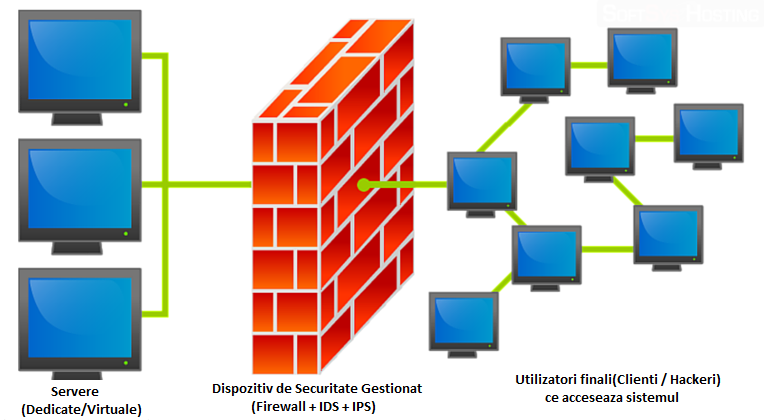
\includegraphics[width=0.6\textwidth]{ips.png}
	\caption{ Administrarea securității unei aplicații }
	\label{fig:ips-example}
\end{figure}

Figura ~\ref{fig:ips-example}  prezintă administrarea securității unei aplicații folosind combinația dintre cele trei sisteme.  \\

În comparație cu sistemele de detecție a intruziunilor care sunt sisteme pasive și scanează rețeaua fără să interfereze cu traficul, sistemele de prevenire a intruziunilor sunt plasate între server și clienți, alterând în mod automat traficul în cazul în care acesta declanșează una din regulile prezente în sistem. Precum sunt prezentate și în articolul  \textbf{What is an intrusion prevention system?} \cite{what_is_ips},  printre funcționalitățile unui sistem de prevenire a intruziunilor se număra:
\begin{itemize}
	\item  Notificarea unui administrator de rețea în cazul în care una sau mai multe reguli sunt declanșate. 
	\item  Oprirea pachetelor considerate malițioase pentru rețea.
	\item  Blocarea unor utilizatori prin excluderea adreselor IP ale acestora. 
	\item  Resetarea unor conexiuni. 
\end{itemize}

În cea ce privește funcționalitățile oferite de un sistem de prevenire a intruziunilor, acestea sunt specifice tipului sistemului. Conform autorului articolului \textbf{Intrusion Prevention System (IPS): Definition \& Types} \cite{ips_types}, Beth Hendricks,  există patru tipuri primare de astfel de sisteme: 
\begin{itemize}
	\item Network-based: Protejează întreaga rețea.
	\item Wireless: Protejează doar rețeaua wireless.
	\item Network behavior: Examinează traficul din rețea.
	\item Host-based: Software cu scopul de a proteja un singur calculator.
\end{itemize}

Sistemele de tipul Network-based(reprezentând și categoria in care se încadrează  \textit{\thesistitle})  presupun implementarea unor senzori în rețea care capturează și analizează traficul ce trece prin acesta. Acești senzori sunt plasați în puncte cheie ale rețelei pentru a putea captura în timp real traficul, iar în cazul interceptării unor activități malițioase să poată interveni imediat, fără să scadă performanța rețelei. Aceste sisteme oferă protecție rețelei indiferent de dimensiunile sau creșterea acesteia, adăugarea de noi device-uri fiind posibilă fără să necesite adăugarea de noi senzori. Adăugarea de noi senzori fiind nevoită doar în cazul în care traficul rețelei depășește capacitatea de procesarea a senzorilor curenți, influențând astfel performanțele rețelei \cite{impl}.

În funcție de nevoi, un sistem de prevenire a intruziunilor poate să ofere diferite opțiuni de protecție pentru diferite părți ale rețelei. Unele sunt capabile să oprească traficul malițios sau să limiteze lățimea de bandă către anumite părți ale rețelei. Conform \cite{ips_sec_types} aceste sisteme pot oferi protecție împotriva următoarelor tipuri de atacuri: 
\begin{itemize}
	\item \textbf{ICMP Storms:}  un volum mare de ecouri ICMP pot să indice activități malițioase precum cineva ce scanează rețeaua. 
	\item \textbf{Ping to Death:}  un utilizator poate să modifice comandă de ping, astfel încât să trimită un număr mare de pachete de dimensiune mare către o destinație țintă pentru a o scoate din uz. 
	\item \textbf{SSL Evasion:}  unele atacuri se pot folosi de criptarea SSL pentru a evita dispozitivele de securitate, întrucât în general acestea nu sunt decriptate. 
	\item \textbf{IP Fragmentation:}  constă în exploatarea faptului că pachetele sunt descompuse în fragmente pentru a satisface cerințele de dimensiune a rețelelor traversate, inundând o destinație țintă cu fragmente false pentru a îi consuma resursele.  
	\item \textbf{SMTP mass mailing attacks:}  un sistem infectat poate să se folosească de email-ul utilizatorului pentru a se răspândi, rezultând într-un trafic mare destinat serverului de mail. 
	\item \textbf{DoS/DDoS attacks:} cu scopul de a face o resursa indisponibilă utilizatorilor, este realizată prin inundarea sistemului țintă cu un număr mare request-uri de la unul sau mai multe(în cazul Dos distribuit-DDoS) sisteme malițioase. 
	\item \textbf{SYN Flood attacks:}  atacatorul trimite un număr mare de pachete de inițiare a unei conexiuni fără să mai răspundă ulterior, epuizând astfel resursele de memorie. 
	\item \textbf{Http obfuscation:}  pentru a evita să fie detectate de anumite sisteme de protecție, unele atacuri folosesc tehnici de ofuscare a request-urilor HTTP. 
	\item \textbf{Port Scanning:}  este folosit pentru descoperi ce porturi sunt deschise pe un sistem, ulterior permițându-i atacatorului să știe ce vulnerabilități ar putea prezenta sistemul. 
	\item \textbf{ARP Spoofing:}  un atacator trimite în rețea pachete false de ARP legându-și propria adresă MAC de adresa IP a unui alt sistem. Ca urmare, atacatorul va primi pachete destinate sistemului cu adresa IP folosită în pachetul de ARP. 
	\item \textbf{CGI Attacks:}  un atacator poate să trimită request-uri malițioase, determinând destinația să trateze request-ul primit ca și cod executabil, oferindu-i atacatorului acces pe sistem. 
	\item \textbf{Buffer Overflow attacks:}  presupune ca atacatorul să depășească limitele unui buffer de lungime fixă, excesul de date ajungând să suprascrie zone adiacente de memorie rezultând în căderea sistemului sau dându-i atacatorului oportunitatea să ruleze cod propriu. 
	\item \textbf{OS Fingerprinting attacks:}  presupune ca atacatorul să descopere ce sistem de operare rulează pe un sistem și folosindu-se de această informație să exploateze vulnerabilități specifice acelui sistem de operare. 
\end{itemize}

Sistemul propus, \textit{\thesistitle}  implementează un sistem de prevenire a intruziunilor folosindu-se de un reverse proxy pentru a intercepta tot traficul care intră și iese din rețea (reprezentând senzorii ce au rol de a captura și analiza traficul) și oferind protecție împotriva a două categorii de atacuri: oprirea de URL-urilor malițioase destinate unei aplicații(protecție împotriva SQL injection) și blocarea adreselor IP cunoscute ca fiind folosite de utilizatori rău intenționați(protecție împotriva adreselor IP ale rețelei Tor). 

Pentru prevenirea atacurilor de SQL injection, se folosește o metodă asemănătoare celei propuse de Eun Hong Cheon, Zhongyue Huang și Yon Sik Lee în lucrarea  \textbf{Preventing SQL Injection Attack Based on Machine Learning} \cite{sqli_how}. Pentru clasificarea request-urilor HTTP în SQL injection sau curate, se folosește un sistem bazat pe machine learning. Acest sistem este antrenat anterior cu date reale, ca și trăsături fundamentale în clasificare, folosindu-se cuvintele cheie și simbolurile specifice limbajului SQL(spre exemplu: SELECT, ADD, DELETE, ", ' etc.). 

\begin{figure}[h]
\centering
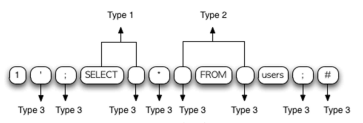
\includegraphics[width=0.6\textwidth]{sqli.png}
\caption{ Tipuri de trăsături ale limbajului SQL }
\label{fig:sql-features}
\end{figure}

Figura ~\ref{fig:sql-features}  prezintă tipurile de trăsături luate în considerare în lucrarea \textbf{Preventing SQL Injection Attack Based on Machine Learning} în raport cu simbolurile sau cuvintele cheie folosite.  


 O altă abordare pentru prevenirea atacurilor SQLI este propusă de Fredrik Valeur, Darren Mutz și Giovanni Vigna în lucrarea \textbf{A Learning-Based Approach to the Detection of SQL Attacks} \cite{sqli_how2}. În această lucrare se prezintă folosirea unui sistem bazat pe detecția de anomalii pentru detectarea atacurilor ce exploatează o aplicație pentru a îi compromite baza de date. Asemeni abordării bazate pe machine learning, acest sistem presupune o fază anterioară de antrenare în care se învață comportamentul normal al utilizatorilor, alcătuind astfel niște profile specifice. Astfel în faza de detecție, comportamentul ce nu coincide cu profilele alcătuite în faza de antrenate, este considerat malițios. 

Pentru prevenirea utilizatorilor de Tor, în general lista de IP-uri este alcătuită din toate IP-urile care au utilizat rețeaua într-un anumit interval de timp, aceasta fiind actualizată periodic. O astfel de abordare este folosită și în cazul marelui firewall al Chinei  \cite{china_tor}  care identifică nodurile la prima accesare a rețelei de Tor. Însă precum precum se evidențiază și în articolul  \textbf{Characterizing the Nature and Dynamics of Tor Exit Blocking} \cite{tor_1} o astfel de abordare nu este cinstită față de unii utilizatori de Tor, întrucât reputația acestora este împărțită între toți utilizatorii. Astfel un nod care este utilizat doar pentru câteva minute sau ore(probabil din motive de curiozitate) poate să ajungă să fie blocat, fiind tratat asemeni cu un nod ce funcţionează de câteva zile. O astfel de discriminare a încercat să fie evitată prin implementarea aleasă a sistemului propus. Pentru realizarea listei de IP-uri blocate se folosește un algoritm ce stabilește o limită de timp minima de funcționare pentru un anumit nod în intervalul a 30 de zile. 


 \section{Tehnici/Tehnologii/Surse folosite}

Pentru realizarea sistemului propus s-au folosit două limbaje de programare: Pyhton2/3(pentru partea de back end) și C\#(pentru partea de front end). În partea de back end a proiectului se realizează implementarea unui reverse proxy pentru a intercepta traficul uneia sau mai multor interfețe, un modul pentru clasificarea request-urilor împotriva atacurilor SQL injection și un modul pentru generarea listei negre de IP-uri ce utilizează frecvent rețeaua Tor. Toate aceste componente sunt realizate prin utilizarea de librării open-source pentru a ușura și eficientiza munca precum:  twisted \cite{twisted}, beautiful soup \cite{btf_soup}, libsvm \cite{libsvm}.

Motivul utilizării atât a limbajului Python3 cât și Python2 este datorat diferențelor de module și librării open-source disponibile pentru cele două limbaje dar și a faptului că suportul pentru Python2 se încheie în anul 2020. Conform documentațiilor oficiale  \cite{python3_doc} și \cite{python2_doc}, dar și articolului \textit{Python 2 to python 3: why, and how hard can it be?} de Tim Grey \cite{why_python3},  între cele două versiuni nu sunt modificări majore, însă în anumite cazuri pot exista librării care să ofere doar suport pentru una dintre acestea. 

În realizarea modulului pentru clasificarea request-urilor împotriva atacurilor SQL injection s-a folosit o colecție de date reale atât de atacuri cât și de trafic curat. Pentru uniformizarea acestor date și pentru a trata tentativele de păcălire a clasificatorului prin codarea unor caractere în valoarea lor în cod hexadecimal (exemplu 'https://www.google.ro /search?q=a' echivalent cu 'https://www.google.ro/search?q=\%61') datele au fost preprocesate și transformate în întregime în coduri hexadecimale  \cite{ascii}.  În procesarea datelor, pentru identificarea trăsăturilor relevant, s-au identificat caracterele specifice limbajului \cite{char_sql} si cuvintele cheie rezervare \cite{key_sql}. Ulterior, pentru antrenarea modelului de support vector machine și pentru clasificarea noilor request-uri s-a folosit software-ul open-source libsvm \cite{libsvm_class}. 
%\newpage
\begin{figure}[h]
	\centering
	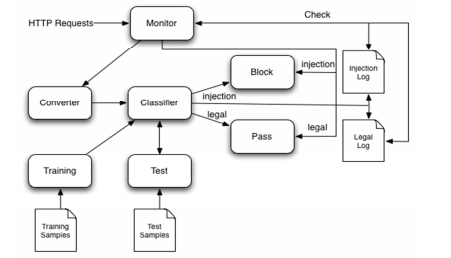
\includegraphics[width=0.5\textwidth]{sql_arh.png}
	\caption{Arhitectura unui sistem de clasificare a request-urilor HTTP}
	\label{fig:sql-arh}
\end{figure}

Figura ~\ref{fig:sql-arh}  prezintă arhitectura unui sistem de clasificare a request-urilor HTTP de un sistem bazat pe machine learning. Structura este prezentată în lucrarea prezentată și anterior  \textbf{Preventing SQL Injection Attack Based on Machine Learning} \cite{sqli_how}.  Acesta structură a reprezentat un model de pornire în realizarea modulului de prevenire a atacurilor SQL injection, implementarea modulului încercând să aducă îmbunătățiri de performanță prin modificarea algoritmului folosit pentru antrenarea modelului de support vector machine, dar și prin filtrarea trăsăturilor propus în lucrare în conformitate cu raportul dintre obișnuința de apariție a acestora atât în request-urile ce intenționează să execute un atac cât și în cele curate. 

Pentru blocarea IP-urilor utilizate de rețeaua Tor s-a folosit un script scris în Python3. Programul interoghează periodic(din 6 în 6 ore) informațiile oferite de \textit{Tor Network Status} \cite{tot_status} identificând astfel nodurile cu un "Uptime" mai mare de 7 zile în parcursul unei luni. Blocarea IP-urilor se realizează prin compararea cu o astfel de listă generată lunar. 

Componenta ce încorporează toate modulele de protecție, este cea de reverse proxy. Aici este monitorizat tot traficul ce vine de pe o anumită interfață(una sau mai multe, în funcție de configurația utilizatorului) și este trecut prin toate modulele disponibile pentru a verifica condițiile de securitate. Pentru testarea dacă o adresă IP este utilizată frecvent de rețeaua Tor, în momentul în care un client dorește să realizeze o conexiune la server-ul protejat de sistem, adresa IP a acestuia este verificată să nu se afle pe lista IP-urilor blocate. Pentru actualitate, lista adreselor IP blocate este actualizată periodic cu adresele IP utilizate frecvent de rețeaua Tor în ultima luna. Modulul de prevenire a atacurilor SQL injection este integrat tot în componenta de reverse proxy, însă evaluarea request-urilor este făcută după realizarea conexiunii între client și server. Request-urile primite de către server sunt tratate asemănător celor folosite pentru antrenarea modulului de support vector machine, însă pentru clasificarea acestora este folosit modulul antrenat în fază inițială și software-ul de prezicere oferit tot de libsvm \cite{libsvm}.
	
	

	





